\chapter{Datenmanagement \& Datenanalyse}

In dem folgenden Kapitel werden einige Technologien, Libaries & Packages, sowie generelle Software gegenübergestellt. Diese werden dann subjektiv bewertet, und die am besten geeignetsten werden für das Projekt verwendet.

\section{Datenmanagement}

	\subsection{Vergleich NoSQL und relational [1]}
		\subsubsection{SQL Datenbanken}
			\begin{itemize}
				\item Typen: Nur eine Art mit kleinen Unterschieden
				\item Data Storage Model: Individuele Einträge werden als Reihen (Rows) in Tabellen gespeichert, wobei jede Zelle spezifische Daten über diesen Eintrag beinhaltet. 
				\item Schemas: Strukur und daten type sind im vorhinein festgelegt. Um diese Datenbank Struktur zu ändern muss diese zunächst offline gesetzt werden.
				\item Skalierbarkeit: Ein einzelner Server muss hierfür mehr Rechenleistung erhalten um größeren Anspruchen nachzukommen. Es ist prinzipiell möglich SQL Datenbanken auf ein verteiltes System zu erstellen, hierfür werden aber sehr gute Kenntnise benötigt.
				\item Data Manipulation: Mittels SELECT, INSERT oder UPDATE
				\item Konsistenz: Gute konsistenz kann prinzipiell in allen gänglichen DBMS konfiguriert werden.
			\end{itemize}

		\subsubsection{NoSQL Datenbanken}
			\begin{itemize}
				\item Typen: Viele verschiedene, bspw. key-value, document-based, oder graph datenbank.
				\item Data Storage Model: Hängt vom Typ der Datenbank ab.
				\item Schemas: Typischerweise dynamich. Einträge können \'on-the-fly\' hinzugefügt werden.
				\item Skalierbarkeit: Bei Bedarf kann ein Administrator einfach mehrere Cloud Instanzen hinzufügen. Die Datenbank an sich verteilt die Information auf die notwendige Server Anzahl
				\item Data Manipulation: Durch Objektorientierte APIs
				\item Konsistenz: Abhängig vom Product
			\end{itemize}

		\newpage
		\vfill
		\subsubsection{Relational vs NoSQL}
		Anhand dem folgenden Graphik kann man prinzipiell eine Entscheidung treffen - diese sollte dann den Ansprechungen entsprechen.
		 
		\begin{figure}[h!]
			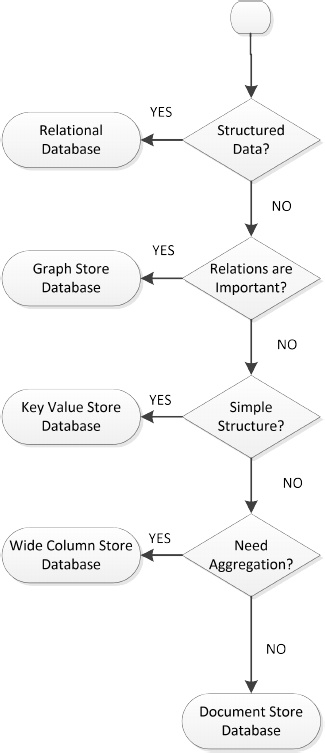
\includegraphics[width=8cm]{decision-flow.jpg}
			\centering
		\end{figure}
		\newpage
		\vfill

	\subsection{NoSQL Datenbanken}

		\begin{tabular} {| l | c | c | c | c | c | c |}
			\hline
			& Cassandra & HBase & MongoDB & Riak & MySQL Cluster & Couchbase		\\ \hline \hline
			Performance &  &	 &  &  &  &  &		\\ \hline
			Supported languages &  &	 &  &  &  &  &	 			\\ \hline
			Documentation &  &	 &  &  &  &  &	 		\\ \hline
			Recent aktivity &  &	 &  &  &  &  &			\\ \hline
			Community &  &  &  &  &  &  &		\\ \hline 
			Usage examples	&  &	&  &  &  &  &					\\ \hline
		\end{tabular}

	\subsection{Rationale Datenbanken}
		
		\begin{tabular} {| l | c | c | c | c | c | c |}
			\hline
			& Sybase & IBM DB2 & Oracle & Microsoft SQL Server & MySQL & PostgreSQL	\\ \hline \hline
			Performance &  &	 &  &  &  &  &		\\ \hline
			Supported languages &  &	 &  &  &  &  &	 			\\ \hline
			Documentation &  &	 &  &  &  &  &	 		\\ \hline
			Recent aktivity &  &	 &  &  &  &  &			\\ \hline
			Community &  &  &  &  &  &  &		\\ \hline 
			Usage examples	&  &	&  &  &  &  &					\\ \hline
		\end{tabular}

	\newpage
	\subsection{Data Mining \& Data Analysis}
	Durch die Sensoren im Auto sowie durch die zusätzlich durch den CarPC angebrachten wird eine enomre Menge an Daten geliefert. All diese Daten ergeben jedoch erst einen \"Sinn\", wenn wir sie mit geeigneten Verfahren analysieren und auswerten können. 

		\subsubsection{Frameworks}

		\begin{tabular} {| l | c | c | c | c | c | c |}
			\hline
			& RapidMiner & WEKA &  R-Programming & Orange & KNIME & NLTK		\\ \hline \hline
			Performance &  &	 &  &  &  &  &		\\ \hline
			Supported languages &  &	 &  &  &  &  &	 			\\ \hline
			Documentation &  &	 &  &  &  &  &	 		\\ \hline
			Recent aktivity &  &	 &  &  &  &  &			\\ \hline
			Community &  &  &  &  &  &  &		\\ \hline 
			Usage examples	&  &	&  &  &  &  &					\\ \hline
		\end{tabular}

	\newpage
	\subsection{Conclusio}
	Anhand der Evaluierung wurde die Auswahl auf die folgenden zwei DBMS Systeme beschränkt: Couchbase (NoSQL) und PostgreSQL (Relational). Da die Anforderungen momentan noch nicht fixiert sind wurde eine relationale und eine NoSQL Variante gewählt (STAND: 02. Okt 2015). In den folgendem Abschnitt gehen wir ein wenig detailierter auf die beiden Systeme ein.

		\begin{table}[htb]
			\begin{tabular}{|l|l|l|}
			\hline
			Name & \textbf{Couchbase} & \textbf{PostgreSQL} \\ \hline
			Description & \begin{tabular}[c]{@{}l@{}}JSON-based document store\\ derived from CouchDB with\\ Memcached-compatible interface\end{tabular} & \begin{tabular}[c]{@{}l@{}}Based on the object relational\\ DBMS Postgres\end{tabular} \\ \hline
			Database model & Document store & Relational DBMS \\ \hline
			Website & www.couchbase.com & www.postgresql.org \\ \hline
			Technical documentation & www.couchbase.com/docs & www.postgresql.docs/manuals \\ \hline
			Developer & Couchbase, Inc. & \begin{tabular}[c]{@{}l@{}}PostgreSQL Global \\ Development Group\end{tabular} \\ \hline
			Initial release & 2011 & 1989 \\ \hline
			Current release & 3.0.3, March 2015 & 9.4.4, June 2015 \\ \hline
			License & Open Source & Open Source \\ \hline
			Server operating systems & \begin{tabular}[c]{@{}l@{}}Linux\\ OS X\\ Windows\end{tabular} & \begin{tabular}[c]{@{}l@{}}FreeBSD\\ HP-UX\\ Linux\\ NetBSD\\ OpenBSD\\ OS X\\ Solaris\\ Unix\\ Windows\end{tabular} \\ \hline
			Data scheme & schema-free & yes \\ \hline
			Typing (data types) & no & yes \\ \hline
			Secondary indexes & yes & yes \\ \hline
			SQL & no & yes \\ \hline
			\end{tabular}
			\caption{Couchbase und PostgreSQL (1)}}
			\label{Couchbase und PostgreSQL (1)}
		\end{table}

		\newpage

		\begin{table}[htb]
			\begin{tabular}{|l|l|l|}
			\hline
			Name & \textbf{Couchbase} & \textbf{PostgreSQL} \\ \hline
			\begin{tabular}[c]{@{}l@{}}APIS and other access\\ methods\end{tabular} & \begin{tabular}[c]{@{}l@{}}Memcached protocol\\ RESTful HTTP API\end{tabular} & \begin{tabular}[c]{@{}l@{}}native C library\\ Streaming API for large objects\\ ADO.NET\\ JDBC\\ ODBC\end{tabular} \\ \hline
			\begin{tabular}[c]{@{}l@{}}Supported programming\\ languages\end{tabular} & \begin{tabular}[c]{@{}l@{}}.NET\\ C\\ Clojure\\ ColdFusion\\ Erlang\\ Go\\ Java\\ JavaScript\\ Perl\\ PHP\\ Python\\ Ruby\\ Scala\\ Tcl\end{tabular} & \begin{tabular}[c]{@{}l@{}}.NET\\ C\\ C++\\ Java\\ Perl\\ Python\\ Tcl\end{tabular} \\ \hline
			Server-side scripts & View functions in JavaScript & user defined functions \\ \hline
			Triggers & yes & yes \\ \hline
			Partitioning methods & Sharding & \begin{tabular}[c]{@{}l@{}}no, but can be realised using\\ table inheritance\end{tabular} \\ \hline
			Replication methods & \begin{tabular}[c]{@{}l@{}}Master-master replication\\ Master-slave replication\end{tabular} & Master-slave replication \\ \hline
			MapReduce & yes & no \\ \hline
			Consistency concepts & \begin{tabular}[c]{@{}l@{}}Eventual Consistency\\ Immediate Consistency\end{tabular} & Immediate Consistency \\ \hline
			Foreign keys & no & yes \\ \hline
			Transaction concepts & no & ACID \\ \hline
			Concurrency & yes & yes \\ \hline
			Durability & yes & yes \\ \hline
			User concepts & \begin{tabular}[c]{@{}l@{}}simple password-based access\\ control per bucket\end{tabular} & \begin{tabular}[c]{@{}l@{}}fine grained access rights\\ according to SQL-standard\end{tabular} \\ \hline
			\end{tabular}
			\caption{Couchbase und PostgreSQL (2)}}
			\label{Couchbase und PostgreSQL (2)}
		\end{table}

